\chapter{FRF Experiment}
\label{sec:frf-experiment}

Diffusion weighted magnetic resonance imaging (dMRI) has been widely used to probe the structure and organisation of brain tissue, with one particular area of focus being the estimation of the orientational distribution of neuronal fibres in a voxel. Many techniques have been developed for estimating this fibre orientation distribution (FOD), a family of which are based on spherical deconvolution.

While there are a variety of spherical deconvolution methods, the central principle is the same - the diffusion weighted signal as a function of the azimuthal ($\phi$) and elevation ($\theta$) angles is modelled as a spherical convolution of the FOD, F($\theta,\phi$), with a kernel (called the fibre response function (FRF)), R($\theta$), the typical diffusion weighted signal from a single fibre population estimated a priori:
\begin{equation}
  S(\theta, \phi) = F(\theta, \phi) \otimes R(\theta) \,.
  \label{eq:spherical_conv}
\end{equation}

By modelling the signal in this way, the FRF is assumed to be the same for all fibres (or fibre populations) in the voxel, meaning that the overall signal is just this FRF summed up across the orientations of all the fibres.
Additionally, this representation cannot properly account for non-straight fibres since an assumption is made that there is no exchange between fibres or, equivalently, between diffusion in different directions.
In essence, this means that the fibres are implicitly assumed to be perfectly straight and pointing a given direction since any deviation from straight (i.e. curved or undulating fibres) would add directions that are dependent on one another.

In practice, however, it is not possible to have a large number of straight fibres pointing in different directions within the same space and maintain a high fibre volume fraction other than in a few simple cases such as planar dispersed cylinders. Ex vivo studies using 3D electron microscopy of mouse corpus callosum have shown than axons are generally not straight, at least in part as a result of having to pack together around one another and other cells.

In this work we use ConFiG, a recently developed white matter numerical phantom generator capable of generating realistic WM morphology, to investigate how realistic packing of fibres affects the diffusion within each fibre and whether the dMRI signal from each fibre is the same, as SD assumes.

\section{Method}
In order to test what impact the complex morphology introduced by packing fibres together has on the individual fibre response functions and how this varies from the straight fibre model used in SD a simulation experiment was performed in a set of numerical phantoms generated using ConFiG. 

\subsection{Phantom Generation}
The fibres generated using ConFiG are not simple straight cylinders since the fibres must bend and bulge to fit around one another. Phantoms were generated for a single bundle of fibres with different amounts of orientation dispersion (OD). A target OD was generated for each phantom using orientations drawn from the Watson distribution [CITE] for $\kappa$ = 2, 6, 10, 15, 20, 50, 100.
A low $\kappa$ means high orientation dispersion, so phantoms with a lower $\kappa$ were expected to have more complex morphology since higher OD means that they must grow around one another more to avoid intersections. A typical $\kappa$, estimated using NODDI [CITE], for the corpus callosum of a healthy Human Connectome Project (HCP) [CITE] subject is $\kappa \sim 6$.

\todo[inline]{Here I want to quantify the microstructural complexity of the phantoms, primarily amount of undulation and amount of beading, to associate with variability in per-fibre FRF}

\subsection{dMRI simulation}
To see how the response function for each fibre is different, the dMRI signal was simulated from each fibre in the phantoms using Camino[cite]. For each fibre 10,000 spins were initialised uniformly intra-axonal space and the simulations were performed using 5000 timesteps. A small set of test simulations were performed using 10$^5$ spins and 10$^4$ timesteps yielding negligibly different signals to these settings, so 10,000 and 5,000 were used for the main simulations. The measurement parameters were $\Delta$ = 28 ms, $\delta$ = 24ms, b = $0,1,2,3,5,10$ ms/$\mu$m$^2$ and 256 gradient directions at each shell. This gives a diffusion time $d_t$ = 20ms and G = 60 mT/m \todo{Get the G} at b = 3000 $\mu$m$^2$/ms, chosen to be a feasible gradient strength on a high-end clinical system. 

To compare to the collection of straight fibres assumption implicit in the spherical deconvolution, a cylinder representing each fibre was generated using the endpoints of each fibre to give the direction and the mean radius of the fibre as the cylinder radius. The signal from each cylinder was generated using an analytical expression [I use NODDI toolbox, find citation for where that analytical expression comes from]. 

\subsection{Signal analysis}
\todo[inline]{complete}

\section{Results}
\begin{figure}
  \centering
  \begin{subfigure}[]{0.32\textwidth}
    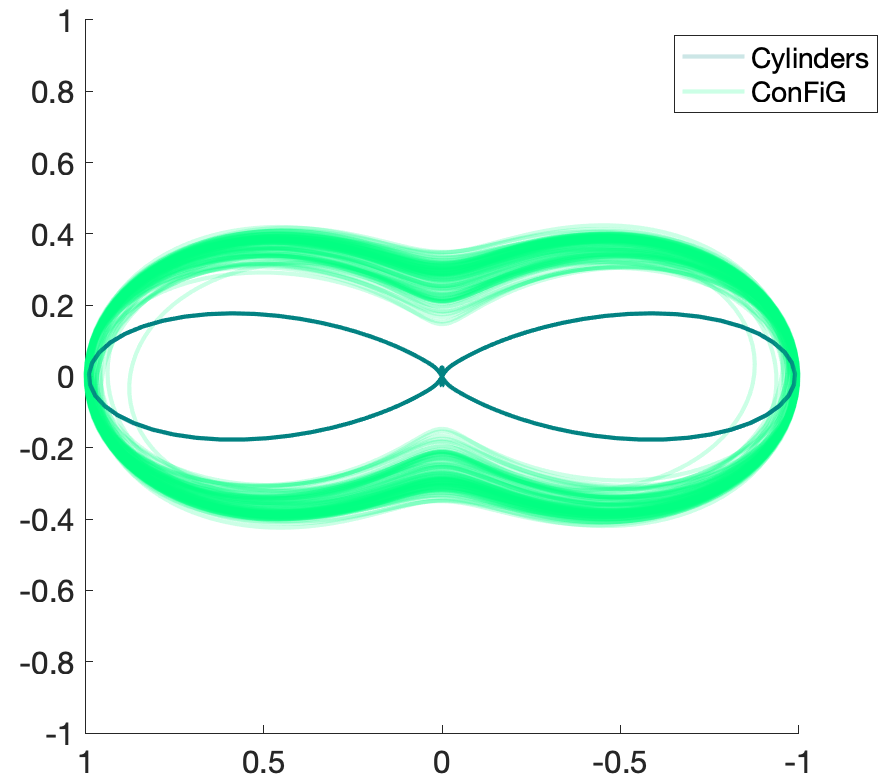
\includegraphics[width=\textwidth]{figures/frf_experiment/kappa_2_b_3000.png}
    \caption{}
  \end{subfigure}
  ~
  \begin{subfigure}[]{0.32\textwidth}
    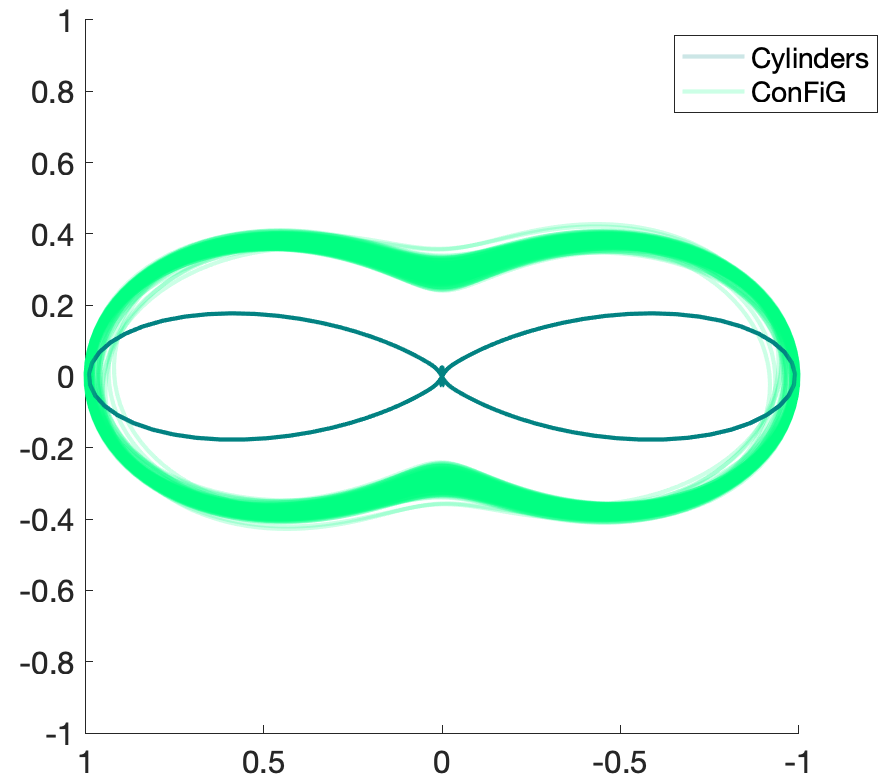
\includegraphics[width=\textwidth]{figures/frf_experiment/kappa_6_b_3000.png}
    \caption{}
  \end{subfigure}
  ~
  \begin{subfigure}[]{0.32\textwidth}
    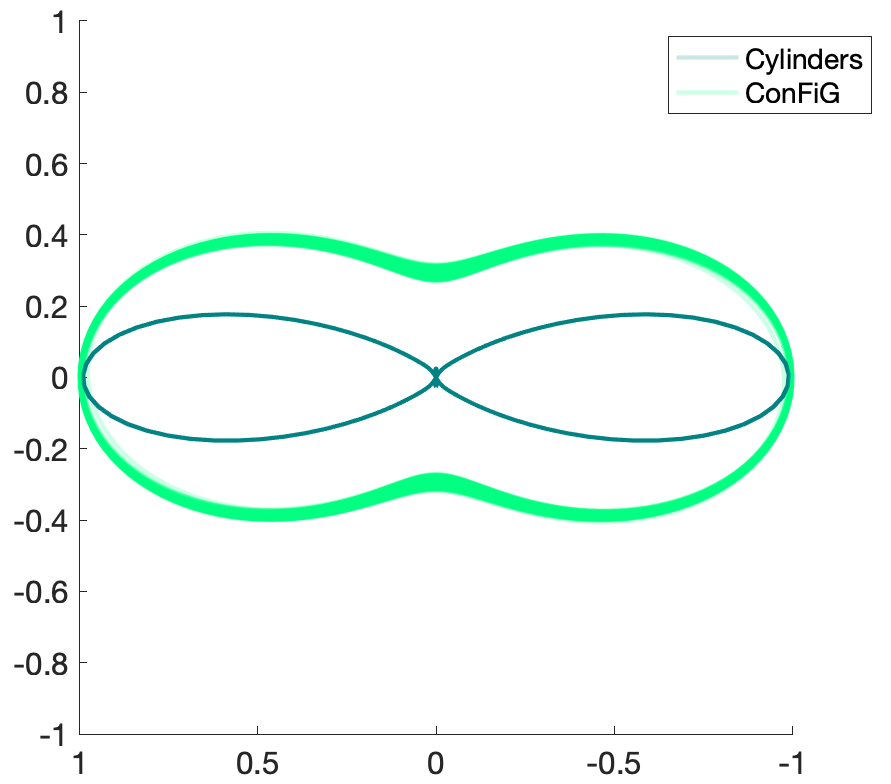
\includegraphics[width=\textwidth]{figures/frf_experiment/kappa_100_b_3000.png}
    \caption{}
  \end{subfigure}

  \caption{Per-fibre FRF at b = 3000 $\mu$m$^2$/ms for $\kappa$ =(a)2, (b)6, (c)100.}
  \label{fig:frf_per_fibre_b3000}
\end{figure}


%%% Local Variables:
%%% mode: latex
%%% TeX-master: "../main"
%%% End:
